\chapter{Proposed approach}

Our primary goal is exploring the effectiveness of probability approaches applied in DeepAR [\cite{2017arXiv170404110S}] for a deep RL agent applied for solving NAS problems.

Leaving alone RL, probabilistic approaches seem to be quite effective for solving hyperparameter optimization tasks. Modern Bayesian optimization approaches showed good results in hyperparameter optimization for image classification problems[\cite{thornton2013auto}; \cite{SnoekLA12}].

Rewards received from a different model of the same architecture built with different hyperparameters form a highly nonlinear response surface [\cite[see]{ZeilerF13}]. How could probabilistic approaches affect the performance of RL agent solving hyperparameter optimization tasks? To answer this question, we would build two RL agents which generate slave CNNs, one with a classical master CNN and another with modified CNN with a Gaussian Layer as it's output and compare the way they learn and transfer knowledge.

To calculate the loss function for the algorithm, we will use MLE of variance for Gaussian modification of CNN and Huber loss for the classical one.

\section{RL agent}

To implement RL agent we heavily rely on the pipeline described in \cite{ZophL16}.

Since there is no physical space $\sset$ for this MDP, we will need to create an abstraction Manager which is responsible for:

\begin{itemize}
\item Generating slave CNN in accordance with actions taken by the agent
\item Evaluate slave CNN for a certain number of epochs
\item Return reward in terms of CNN accuracy
\end{itemize}

Since there is no initial state, random action is generated in order to provide proper state transition $\Tdef$.

RNN was used as a backend for RL algorithm in the original paper [\cite{ZophL16}] but we use simple CNN to make integration of Gaussian Layer easier.

Since RL needs a finite set of actions $aset$ we are limiting hyperparameters options to a set of predefined values.

Each epoch RL agent can either explore random action or predict one using backend CNN. After the reward would be returned, state transition should be stored in the replay memory. Random batches of those transitions should be taken and used as input to update master (backend) CNN (see \ref{fig:dqn}).

Since there is no actual next state for the controller, transition objects would contain the previous state, action taken and reward received.

Since master CNN actually performs a regression task, we also use a converter that converts its outputs into actions that should be taken next. Obviously, the output layer could be modified to make this CNN solve a classification problem, but this trick was used in order to appropriately evaluate outputs of Gaussian Layer.

\begin{figure}[!htb]
  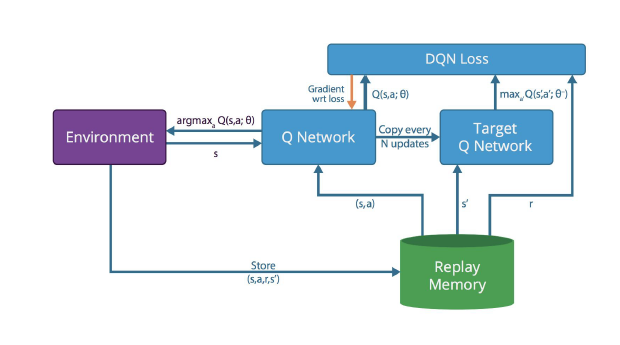
\includegraphics[width=\linewidth]{images/dqn.png}
  \caption{General overview of DQN RL architecture}
  \label{fig:dqn}
\end{figure}


\subsection{Exploration and exploitation}

Since the action space is limited, during experiments we've observed a tendency of the algorithm to overfit. In order to resolve this, we use two different ways to handle exploration over exploitation dilemma:

\begin{itemize}
\item Decaying random effect occurrence in epsilon-greedy approach 
\item Applying UCB to received reward
\end{itemize}

Both methods were evaluated during experiments.

\section{Master CNN}

Master CNN is used as a backend for the RL agent. Since neural networks are universal function approximators, we can use one to make a prediction of the reward received for taking an action.

This CNN takes in a batch of transition objects. Its outputs are of the size of action space. In effect, the network is trying to predict the expected return of taking each action given the batch of transitions in the classic approach.

In the updated approach this network outputs a $\mu$ and $\sigma$ of Gaussian distribution of expected return of taking each action.

\subsection{Gaussian layer}

When it comes to RL algorithms, scoring becomes very important and may have a big impact on action taken by the controller - \cite[see][]{tilmann}

If master CNN in RL agent is solving a regression problem (which is exactly our case) this CNN would use backpropagation to update its weights (as noted above) in a way that error metrics of a test set would be minimized. Originally outputs of the last layer would be real values - in our case, values that determine the actions that would be taken by the controller.

Those values obviously depend on input and weights. In order to receive a Gaussian distribution, we would need to modify the last layer so that it would return the mean and variance of the output variable, which is enough to describe a Gaussian distribution of this variable. This allows us to bring a prediction uncertainty into the outputs of CNN. As described in \cite{2017arXiv170404110S} this requires also another approach to the computation of loss function.

We are using Gaussian distribution instead of single values because we need to have a measure of uncertainty of prediction of output. The underlying idea is that RL agent should benefit from playing actions with lower uncertainty.

For these needs, any other distribution could be obviously used. DeepAR [\cite{2017arXiv170404110S}] allows users to choose Gaussian, Student T and beta distributions. We've chosen Gaussian distribution for the needs of this project, but any other distribution of real-valued variables could be used with an appropriate likelihood loss function.

\section{Slave CNN}

Slave CNN is a CNN generated by the controller. It could be of any architecture, however, in experiments, the number of hidden layers was restricted to 4 hidden convolutional layers and one GlobalAveragePooling layer.

Here is code listing of slave CNN Model implemented in TensorFlow:

\begin{verbatim}
ip = Input(shape=(28, 28))
x = Conv2D(filters_1, (kernel_1, kernel_1), activation='relu')(ip)
x = Conv2D(filters_2, (kernel_2, kernel_2), activation='relu')(x)
x = Conv2D(filters_3, (kernel_3, kernel_3), activation='relu')(x)
x = Conv2D(filters_4, (kernel_4, kernel_4), activation='relu')(x)
x = Dense(100, activation='softmax')(x)
model = Model(ip, x)
\end{verbatim}

\begin{figure}[!htb]
  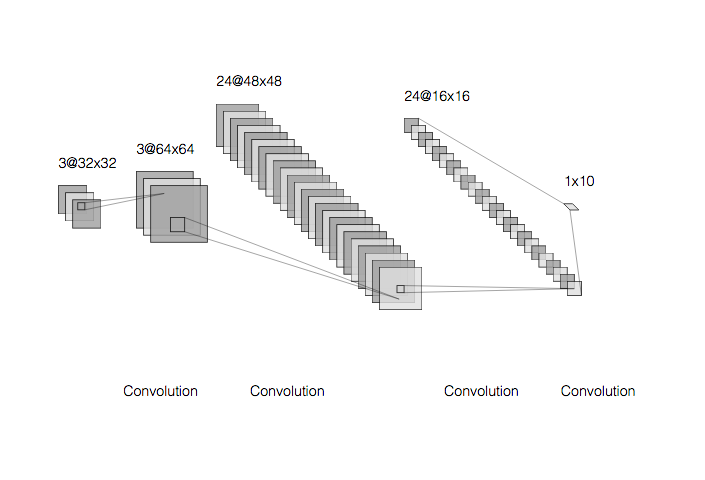
\includegraphics[width=\linewidth]{images/slave-example.png}
  \caption{Example of slave CNN architecture that could be generated by RL agent for CIFAR10 dataset}
  \label{fig:slave}
\end{figure}


